\documentclass[a4paper,12pt]{report}

\usepackage[utf8]{inputenc}
\usepackage[T1]{fontenc}
\usepackage[french]{babel}
\usepackage{url}
\usepackage{wrapfig}
\usepackage{listings}
\usepackage{makeidx}
\renewcommand{\thesection}{\Roman{section})}
\renewcommand{\thesubsection}{\arabic{subsection})}
\renewcommand{\thesubsubsection}{\arabic{subsection})}
\usepackage{xcolor,graphicx}
\usepackage[top=0.6in,bottom=0.6in,right=1in,left=1in]{geometry}
\makeindex
\begin{document}
\begin{titlepage}

\begin{center}
	\begin{minipage}{2.5cm}
	\begin{center}
		
\includegraphics[width=2.5cm,height=1.7cm]{image/iut.jpg}
		
	\end{center}
\end{minipage}\hfill
\begin{minipage}{10cm}
	\begin{center}
	\textbf{ UNIVERSITÉ DE MONTPELLIER}\\[0.1cm]
    \textbf{INSTITUT UNIVERSITAIRE DE TECHNOLOGIE}\\[0.1cm]
    \textbf{BEZIERS}
	\end{center}
\end{minipage}\hfill
\begin{minipage}{2.5cm}
	\begin{center}
		
\includegraphics[width=2.3cm,height=2.5cm]{image/um}
	\end{center}

\end{minipage}
%\includegraphics[width=0.6\textwidth]{logo-isae-supaero}\\[1cm]
\textsc{\Large }\\[1.5cm]
{\large \bfseries Rapport de stage}\\[0.5cm]
{\large En vue de l'obtention du diplôme}\\[1cm]

{\huge \bfseries \uppercase{Diplôme universitaire de technologie} \\[0.5cm] }
{\large \bfseries Filière : Réseaux informatique et télécommunication}
\textsc{\Large }\\[1cm]

% Title
\rule{\linewidth}{0.3mm} \\[0.4cm]
{ \huge \bfseries\color{blue!70!black} Mise en place d'un outil de reporting  \\[0.4cm] }
\rule{\linewidth}{0.3mm} \\[1cm]
{\large \bfseries Organisme d'accueil : Aberia Télécommunication}\\[1cm]
 
\includegraphics[width=0.3\textwidth]{image/aberia}\\[1cm]
% Author and supervisor
\noindent
\begin{minipage}{0.4\textwidth}
  \begin{flushleft} \large
    \emph{\color{orange!80!black}Réalisé par :}\\
    Issa-Mohamed \textsc{Abdoulkarim}\\
  \end{flushleft}
\end{minipage}%
\begin{minipage}{0.5\textwidth}
  \begin{flushright} \large
    \emph{\color{orange!80!black}Sous la direction de :} \\
    Pr.~Lionel \textsc{Cucala} (IUT)\\
    M. Stephane \textsc{VIE} (ABERIA)\\
  \end{flushright}
\end{minipage}\\[1cm]

\color{black}
\centering

% Bottom of the page
{\large \color{orange!80!black}{Année universitaire}\\ \color{blue!80!black}2019/2020}

\end{center}
\end{titlepage}

%%%%%%%%%%%%%%%%%%%%%%%%%%%%%%%%%%%%%%%%%%%%%%%%%%%%%%
%               PAGE VIDE
%%%%%%%%%%%%%%%%%%%%%%%%%%%%%%%%%%%%%%%%%%%%%%%%%%%%%%
\newpage
\strut 
\newpage

%%%%%%%%%%%%%%%%%%%%%%%%%%%%%%%%%%%%%%%%%%%%%%%%%%%%%%%
%les remerciement
%%%%%%%%%%%%%%%%%%%%%%%%%%%%%%%%%%%%%%%%%%%%%%%%%%%%%%%
~
\vfill
 
je tients à remercier mon tuteur de stage de m'avoir .....
 
\vfill

%%%%%%%%%%%%%%%%%%%%%%%%%%%%%%%%%%%%%%%%%%%%%%%%%%%%%%
%           Sommaire
%%%%%%%%%%%%%%%%%%%%%%%%%%%%%%%%%%%%%%%%%%%%%%%%%%%%%
\newpage



\setcounter{tocdepth}{2}
\renewcommand{\contentsname}{Sommaire}
\tableofcontents

\newpage
%%%%%%%%%%%%%%%%%%%%%%%%%%%%%%%%%%%%%%%%%%%%%%%%%%%%%%%%%%%%%%%%%%%%%%%%%%%%%%%%%%%%                                        début 
%%%%%%%%%%%%%%%%%%%%%%%%%%%%%%%%%%%%%%%%%%%%%%%%%%%%%%%%%%%%%%%%%%%%%%%%%%%%%%%%%%%
\section{INTRODUCTION}
\paragraph*{}

              L'analyse des données des entreprises représente fortement un aspect important pour leur développement. De  nos jours, toutes les entreprises font de l'analyse de données pour évaluer leur qualités de services ou leur évolution. Ces analyses leur permettent de tirer des conclusions importantes sur une domaine précise de l’entreprise ou adopter une autre stratégie. Elle est de plus en plus perçue comme un véritable outil incontournable pour accroître  la performance de l’entreprise. Selon une article du KGMP  intitulé « L’analyse des données, un enjeu de confiance et de gouvernance pour les dirigeants », il affirme que : < Près de la moitié des dirigeants interrogés l’utilisent pour analyser les données clients existantes, trouver de nouveaux clients et développer de nouveaux produits et services. Les dirigeants français sont les plus enclins à établir des plans de développement sur l’analyse prédictive (45 \% vs. 24 \% dans le monde) et la visualisation exploratoire (49 \% vs. 21 \% dans le monde).> Cela relève l’importance de l’annale des données quelque soit données client ou données interne à l’entreprise.\newline\newline 
       
       A son tour, afin  d’améliorer sa qualité de service, Aberia veut mettre en place un système de reporting leur permettant de suivre en temps réel l'évolution de leur activité.  Ce système va leur fournir des statistiques cohérentes et fiables sur l'évolution des tickets client afin d'améliorer leur gestion de ticket. En plus, elle fournira, aussi, des rapports quotidien, mensuel  et annuel sur les performances des agents de leur centre d’appel. Enfin, ce système va permettre, également, aux employés situés dans le pôle commercial d’avoir à leur tour des statiques sur leur travail. Ces statiques vont leur permettre d’adopter une nouvelle stratégie en leur faveur. Ainsi, dans une période de 10 semaines, ma mission était de réaliser ce système et l'implémenter sur l’infrastructure d’Aberia tout en respectant les fonctionnalités et les limites du projet. 
\newpage
\section{PRÉSENTATION DE L’ENTREPRISE }
\subsection{IDENTITÉ DE L’ENTREPRISE}
\paragraph*{}

\begin{tabular}{|c|c|}
\hline
Chiffre d’affaires  & 3.7 Millions d’euros \\
\hline
Nombre d’employés & 33 \\
\hline
SIRET & 39342108600041\\
\hline
Collaborateurs  & 31 \\
\hline
Date de création & 1994\\
\hline
Siège social & Béziers\\
\hline
Adresse &229 RUE ALPHONSE BEAU DE ROCHAS 34500 BEZIERS \\
\hline
\end{tabular}
\subsection{Représentation hiérarchique de l’entreprise}
\paragraph*{}

     J’ai travaillé sous les instructions de Stephane VIE, responsable infrastructure et sécurité,  pendant tout mon stage chez Abéria.
\begin{figure}[!h]
\begin{center}
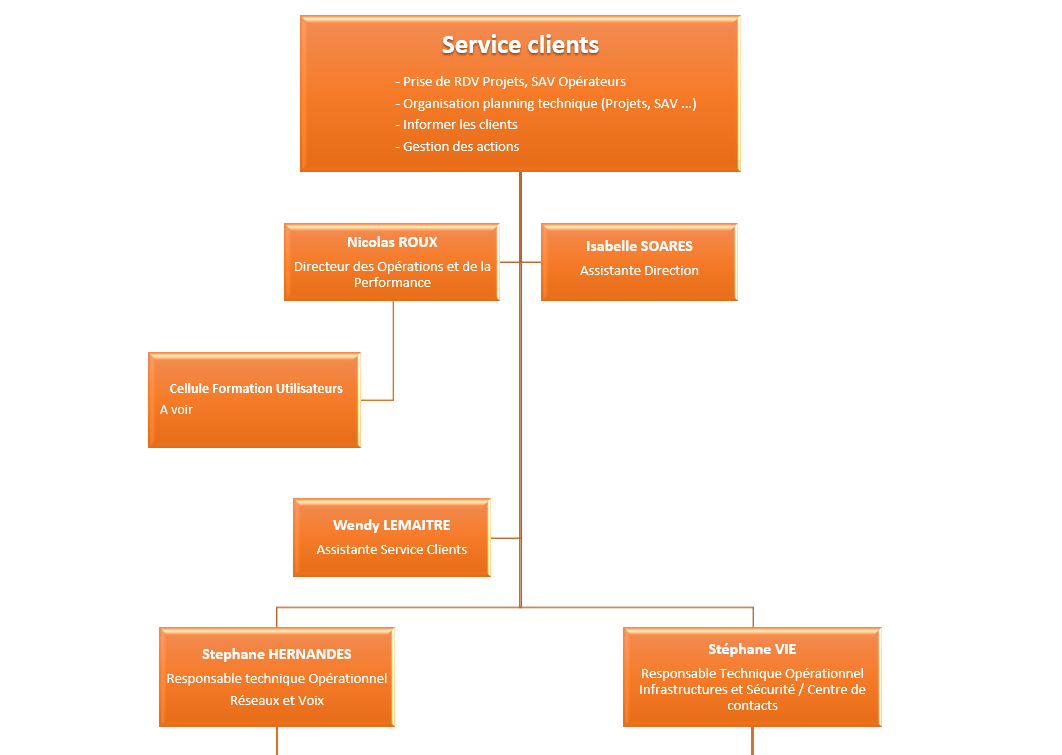
\includegraphics[width=20cm]{image/hierarchi.png}
\end{center}
\caption{Composition de l'entreprise ABERIA}
\label{Photo d'illustration}
\end{figure}
\subsection{Domaine d’activité}
\paragraph*{}

        Aberia est une société basée sur les domaines de la télécommunication, plus précisément  la téléphonie IP(internet protocole). 
        Elle assure plusieurs services à différents clients.\newline
       
       D’abord,  ABERIA évolue dans le domaine de la téléphonie d’entreprise : installation de matériels numéris , Interconnexion de réseau en voix sur ip et data, téléphonie sans fil DECT Wifi Fi, câblage, serveurs vocaux, éditeurs de taxation, Messageries unifiées et service de maintenance.\newline
       En suite, Elle propose des services d'études et de conseils dans les domaines suivants :
\newline
\begin{itemize}
 \item    Convergence voix / Data 
 \item   Interconnexion de réseaux voix \& données 
 \item   La mobilité voix \& data 
 \item  Les Centres d’appel et contres de contacts 
 \item  Les Serveurs vocaux et messageries unifiées 
 \item L’intégration de solutions en mode hospitalier 
\end{itemize}

\paragraph*{}
       Elle ne s’arrête pas là,  Aberia propose aussi des services d'intégration et d'assistance globale.\newline
       
       Enfin, Aberia est une entreprise certifiée au plus haut niveau sur l’ensemble de la gamme de produits, elle  propose des solutions de constructeurs reconnus au niveau mondial.
\subsection{Les partenaires}
\paragraph*{}
Aberia travail en etroite collaboration avec des société mondialement reconnu. \newline Ces collaborateurs sont repartis en 3 groupes : 

\subparagraph{QUADRENA\newline}
      c’est une façon d’entreprendre réfléchie, novatrice et unique dans le Biterrois. Elle repose sur l’enthousiasme et le défi des ces 4 sociétés qui ont choisie aujourd’hui de lier leur avenir économique. 
      Il s’agit d’Aberia, absys informatique, burospace et elit bureautique. 
\subparagraph{CONSTRUCTEUR\newline}
Aberia travaille en etroite collaboration avec les entreprise suivantes : \newline

\begin{itemize}
 \item CISCO
 \item Alcatel*Lucent
 \item Lifesize
 \item Ruckus
 \item Mitel
\end{itemize}

\subparagraph{GROUPE CONVERGENTE\newline}

Le Groupe Convergence est un réseau de sociétés professionnelles indépendantes, expertes dans les métiers des télécommunications, de l’informatique et des services.

\subsection{Projet en cours}
\paragraph*{}
Aberia travaille actuellement sur des projets innovent et intéressant. Ces sont projets sont :

\begin{itemize}
 \item                   Solution voix en mode Saas
                         \item Sécurisation des systèmes d’informations
                        \item  Opérateurs
                      \item Centrex
                        \item Centre d’appel (partenaire Gold référencé auprès de Mitel au niveau national)
                        \item Gestion des rapports statistiques sur les centre d’appels.
\end{itemize}


%%%%%%%%%%%%%%%%%%%%%%%%%%%%%%%%%%%%%%%%%%%%%%%%%%%%%%%%%%%%%%%%%%%%%%%%%%%%%%%%%%%%                            carde et mise en place du projet
%%%%%%%%%%%%%%%%%%%%%%%%%%%%%%%%%%%%%%%%%%%%%%%%%%%%%%%%%%%%%%%%%%%%%%%%%%%%%%%%%%%
\section{Cadre et mise en place des projets}
\subsection{Environnement et organisation du travail}

\paragraph*{}
            j’ai effectué la totalité de mon stage en télétravail. Les horaires ont été 8H30-12h et 14h-18h30 du lundi au vendredi.
           Durant la période de mon stage, mon tuteur me passait un coup de fil le matin afin
           de me donner les instructions. En début d’après midi, il m’appelait encore, afin de voir
           l’évolution des travaux.
           En fin de journée, je devrais lui envoyer un rapport détaillé des taches que j’ai effectué.
\subsection{Cadre du projet}

\paragraph*{}
  Le but du projet est de mettre en place, en 10 semaines, une plate-forme de reporting afin de consulter l'évolution des travaux en temps réel.\newline 
  Ces statiques seront faites sur 3 services de la société :  \newline
 
\begin{itemize}
\item Service technique 
\item Centre d’appel
\item Services commercial \newline
\end{itemize}
La plate forme sera visible qu’en interne. Cette à dire dans le réseaux (IP) de l’entreprise.
\subsection{Fonctionnalités attendu}
\paragraph*{}
La plate-forme doit répondre aux problématiques suivante : 

\subparagraph{ En terme de statistique\newline}

Les statistiques des techniciens, commerciaux et du centre d’appel doivent être reparties en 4 grandes catégories :\newline

\begin{itemize}
 \item Statistique annuelles
 \item Statistique mensuelles
 \item Statistique hebdomadaire
 \item Statistique journaliers 
\end{itemize}


\subparagraph{Compte et Sécurité\newline\newline}
la plate-forme doit permettre aux salariés de se connecter, avec un compte personnel, afin d'observer les statistiques relatives à leurs équipes de travail. Ainsi, une authentification et une restriction des droits doit être mis en place. Aberia dispose un serveur d’authentification LDAP (Lightweight Directory Access Protocol) qui sera mis à disposition dans le cadre de se projet.

\subparagraph{Visualisation et Exportation des résultats\newline\newline}

                      Les résultats des statistiques sont parlants lorsqu’ils sont affichés avec des diagrammes ou histogrammes. Cela permet d’avoir une facilité dans la visualisation des données. Ainsi, dans ce projet les résultats des statiques doivent être affichés avec des diagrammes, histogrammes … . \newline
           
           La plate forme doit permettre aux utilisateurs  de se partager les résultats par mail  et de mettre des alertes sur des statistiques importantes. Elle doit aussi permettre aux différents utilisateurs d’exporter les résultats, au minimum, en excel ou en PDF. 
             
\subsection{Étude du projet}

\subsubsection{Planification du projet (Diagramme de Gant)}
\paragraph*{}
Afin d’arriver à finir le projet dans les meilleurs délais, Nous, moi et mon tuteur, avons élaboré un diagramme de Gant(annexe …).	  

\subsubsection{Recherche d’un outil de Reporting (Open Source)}

Il existe plusieurs outils  informatiques, Open Source (c’est-à-dire dont le code source est modifiable), permettant de faire du reporting. Mon tuteur de stage en a sélectionné  quelques uns et me les a transmis. J’ai étudié attentivement les documentations de ces outils  en tenant compte des fonctionnalités demandées, des limites invoquées dans le cahier des charges et des coûts en terme de ressources.\newline

Ces outils sont :
\newline
\begin{itemize}
 \item  BIRT
 \item JSREPORT
 \item HELICALINSIGHT
 \item METABASE
 \item KNOWAGE-SUITE
\end{itemize}

\paragraph*{}

               Après analyse et test de ces derniers, j’ai choisis l’outil Metabase.\newline
               
               En effet, Metabase répond aux  critères de sélection mis en avant ci-dessus. 
               Elle possède une particularité sur l’affichage des résultats : les histogrammes, digrammes … sont déjà pré-programmés. 
               Ainsi, nous pourrons personnalisé l’affichage des résultats en utilisant les options fournis par Metabase. Cela représente un énorme gain de temps.
               Donc, avec cet outil, seul les requêtes SQL seront programmées. Contrairement à certains outils qui demandent un effort sur la conception, en java script, des diagrammes.\newline    
               
               Cette solution est approuvé par mon tuteur.  Dès lors, je me suis mis sur le déploiement de cet outil sur les serveurs de l’infrastructure Aberia.  Il s’agit d’un serveur tournant sous CentOS (Community enterprise Operating System) : un système d’exploitation et  distributeur linux. 
      
\subsubsection{Procédure d’installation de Metabase}
\paragraph*{}           
           Après avoir réussi à installer et configurer l’outil Metabase, j’ai rédigé une documentation personnelle qui mettait en avant surtout les problèmes rencontrés au moment de l’installation (Voir annexe 3). Cette documentation est par la suite réutilisée par mon tuteur lors du déploiement de cette solution chez un client( on en reviendra). 
\section{Mise en plce du projet}

\subsection{statistique du service technique}
\paragraph*{}

Le système de gestion de ticket de la société Aberia est basé sur un ERP (Enterprise Resource Planning) : progiciel permettant de gérer l'ensemble des processus d'une entreprise en intégrant l'ensemble de ses fonctions, dont la gestion des ressources humaines, la gestion comptable et financière, l'aide à la décision, mais aussi la vente, la distribution, l'approvisionnement et le commerce électronique (wikipedia). Leur ERP est appelé Atheneo. Il s’agit d’un progiciel fourni par une société d'éditeur de logiciel il y a à peine quelques années. 

\subsubsection{ANALYSE DE LA BASE DE DONNÉE}

\paragraph*{}
                Afin de pouvoir travailler sur la base de données, j’ai procédé à un reverse engineering : activité qui consiste à étudier un objet pour en déterminer le fonctionnement interne ou la méthode de fabrication(wikipedia).\newline
               
               L’ERP tourne avec  un SQL server : système  de gestion de base de données. 
               Avec  l’outil  draw.io, j’ai procédé à l’analyse de la base de donnée. Cette analyse était basé sur deux tables principales. En base de données, une table est une structure interne d’une base de données qui permet de stocker des informations. Il s’agit de la  tables INCIDENT et la tables INFO\_\ INCIDENT.\newline 
               
               La table INCIDENT est la table qui enregistre les incidents ( ticket) envoyé par les clients. La tables INFO\_\ INCIDENT est celle qui enregistre le sicle de vie d’une incident(ticket) : modification, affectation, réouverture …. \newline
               
               L’outil drawo.io m’a permis de modéliser ces deux tables tout en remontant les clés étrangers de ces deux tables (Annexe 2). Dans une base de données, une clé primaire est une valeur unique qui permet d'identifier un élément dans une table. Étant donnée  qu’une base de donnée comprend plusieurs tables, ces dernières peuvent être liées. Ces liaisons se font par les clés primaires des tables. Une clé primaire d’une table injectée dans une autre table est dans ce contexte appelée clé étrangère. 
               Après cette analyse, Cela m’a donné une bonne vision de ces deux tables ce qui  m’a permis de faire mes Requêtes SQL( langage de programmation orienté base de données)  avec une plus grande facilité.\newline 
               
               A partir de ce moment, j’ai commencé par voir le fonctionnement de l’ERP. j’ai étudié dans les millimètres près les fonctionnalités de ce ERP, sous le pilotage de mon tuteur de stage. j’ai pris le temps d’observer les scénarios effectués lors d’un traitement de ticket. Après cela, j’ai commencé à effectuer les requêtes SQL.
                     
\subsubsection{Conception des requêtes SQL}

\paragraph*{}

Les statistiques souhaité par Aberia sont les suivants :\newline 

\begin{itemize}
 \item Nombre de tickets créés 
 \item Nombre de tickets sur tech Hotline 
 \item nombre de ticket en cours par priorité 
 \item Nombre de ticket non sur tech hotline 
 \item Nombre de ticket en cours par tech
 \item Nombre de ticket résolu par tech 
 \item Nombre de ticket clôturé par statut
 \item Top 10 des clients par tickets créés
 \item Nombre de Relance client
 \item Top 10 des clients dont les tickets sont résolus 
 \item Nombre de ticket réouvert
 \item Nombre de ticket data de deux jours.
\end{itemize}

\paragraph*{}
               Ces statistique seront structurées par jour, semaine, mois et année comme il était évoqué dans les attentes. 
               j’ai écrit les requêtes SQL répondant à ces questions tout en plaçant les résultats sur un tableau de bord avec des histogrammes et des diagrammes. Les requêtes SQL sont dans l’annexe 4.
\subsubsection{Résultats}

\paragraph*{}
Ce premier projet a eu un succès. Les statiques demandées par Aberia sont mis en place. La direction et les techniciens pourront, enfin, avoir leurs statiques sur leur écrans. 
\begin{figure}[!h]
\begin{center}
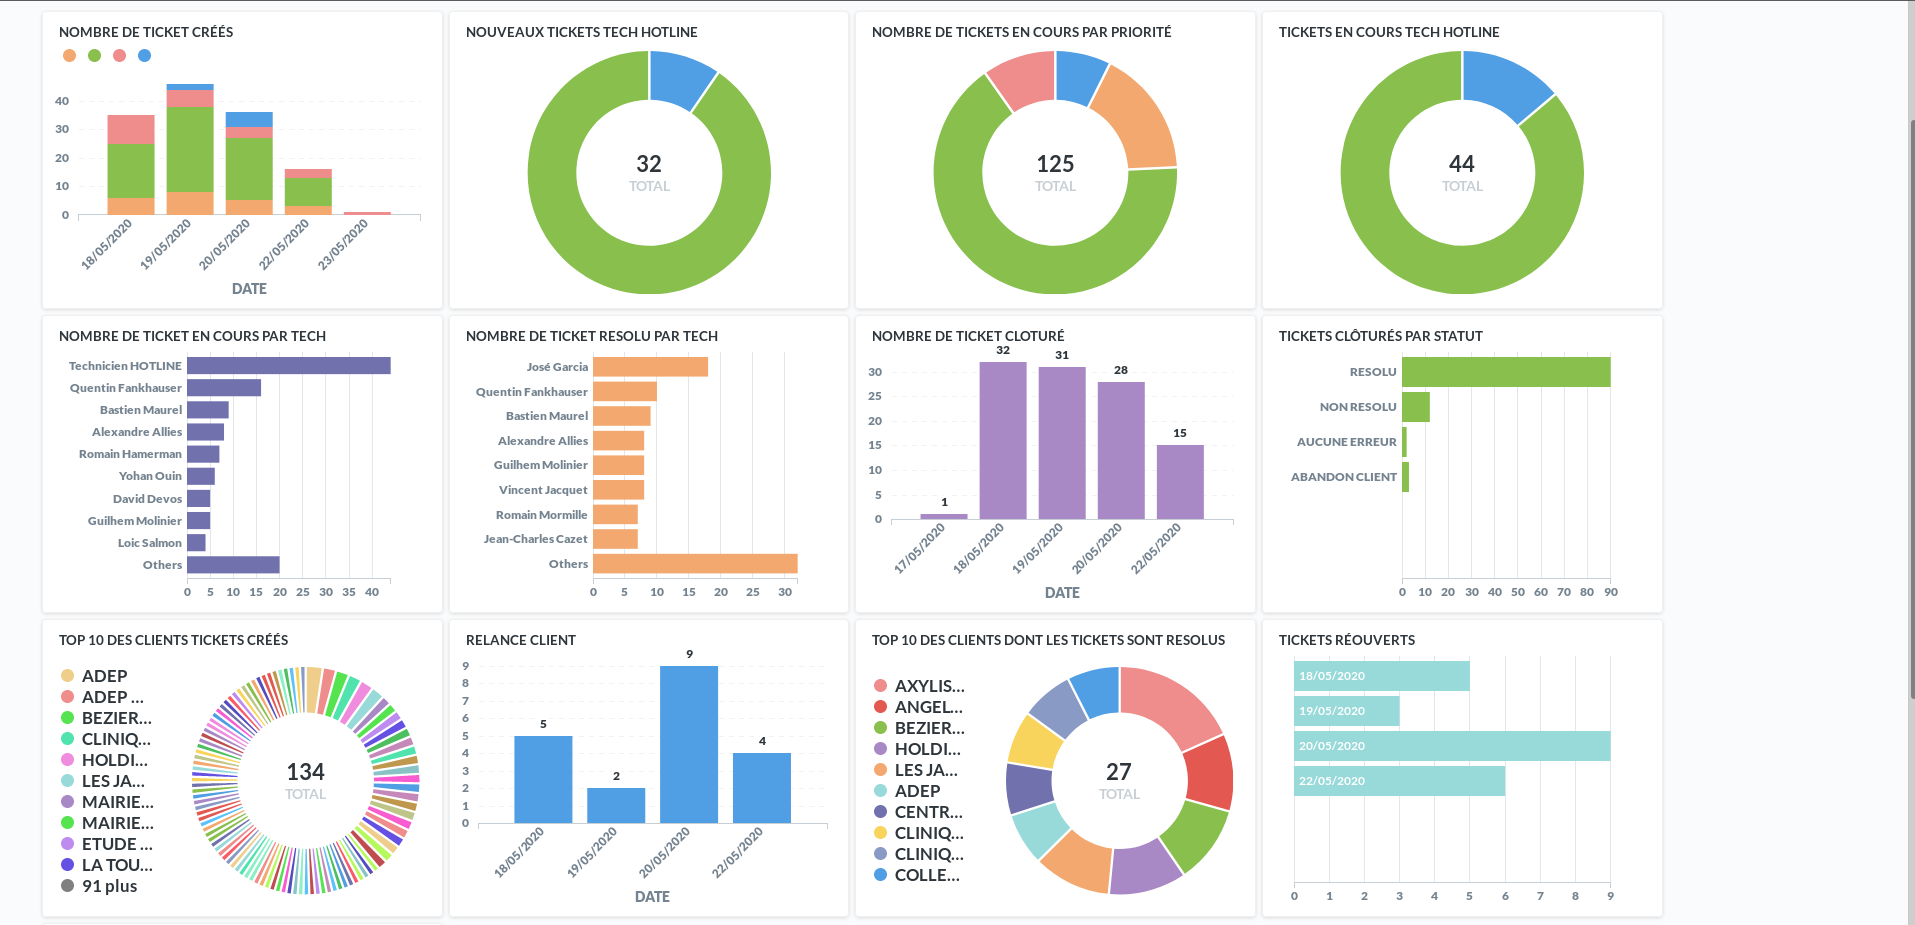
\includegraphics[width=20cm]{image/projet1.png}
\end{center}
\caption{Photo d'illustration des statiques journaliers}
\label{Photo d'illustration}
\end{figure}

\subsection{Statistique sur les centre d’appels}

\paragraph*{}
               Dans ce nouveau projet, l’essentiel est de faire des statiques sur les performances des agents et des files d’attente.\newline  
               Aberia utilise un centre de contacte au nom de MICC (MiContact Center) : un logiciel de gestion d’appel. Ce dernier possède une base de donnée qui en registre tout les événements des agents à savoir le nombre d’appels émis, reçu … etc .\newline 
               MICC tourne avec un SQLserver express : un gestionnaire de base de donnée.
       
\subsubsection{Analyse de la base de donnée}

\paragraph*{}

                   Comme dans le premier projet,  j’ai étudié la composition et l’organisation des données. Le Micc propose des VUES. Une vue, dans une base de données, est une synthèse d'une requête d'interrogation de la base. On peut la voir comme une table virtuelle, définie par une requête(wikipedia). Ainsi, dans ce projet, j’ai travaillé avec des vues et non avec des tables, directement.\newline
                   Dans ce projet, j’avais la documentation officielle. De la composition à l'exécution de la requête SQL, les informations étaient claires et compréhensibles. Ainsi, j’ai suivi cette documentation dans la conception de mes requêtes SQL. 

\subsubsection{Conception des Requêtes SQL}

\paragraph*{}

       Les statiques souhaitées par Aberia sont les suivantes  : 
\begin{itemize}
 \item Les performances des agents.
 \item Les performances des files d’attente.\newline 
\end{itemize}

       Comme dans le projet précédent, ces informations seront organisées par  Années, mois semaines et  jours . Les requêtes SQL répondants à ces problématiques se trouvent sur l’annexe(…). 
\subsubsection{Résultats}

\paragraph*{}
                   Après avoir mis en place les requêtes SQL, j’ai lancé et suivi les tests.\newline 
                   Le projets à bien été réussi. Il est mis en place sur les locaux d’Aberia et à certains clients. 

\begin{figure}[!h]
\begin{center}
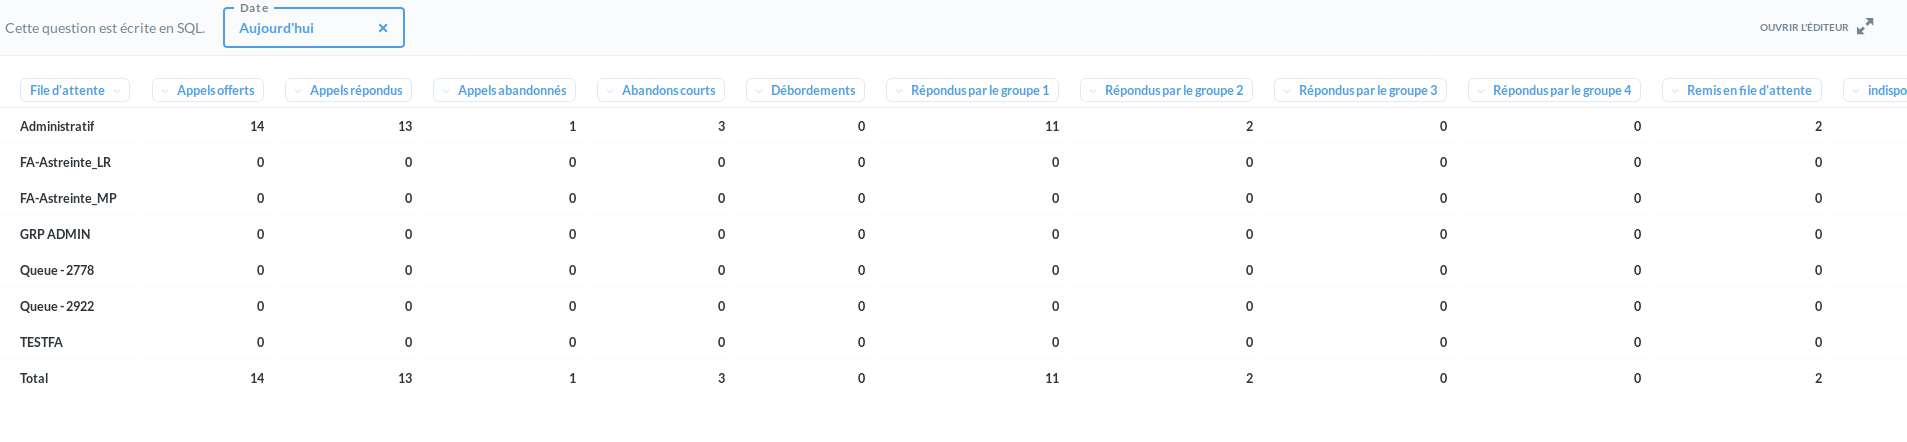
\includegraphics[width=20cm]{image/PROJET2a.png}
\end{center}
\caption{Photo d'illustration des statiques journaliers}
\label{Photo d'illustration}
\end{figure}

\begin{figure}[!h]
\begin{center}
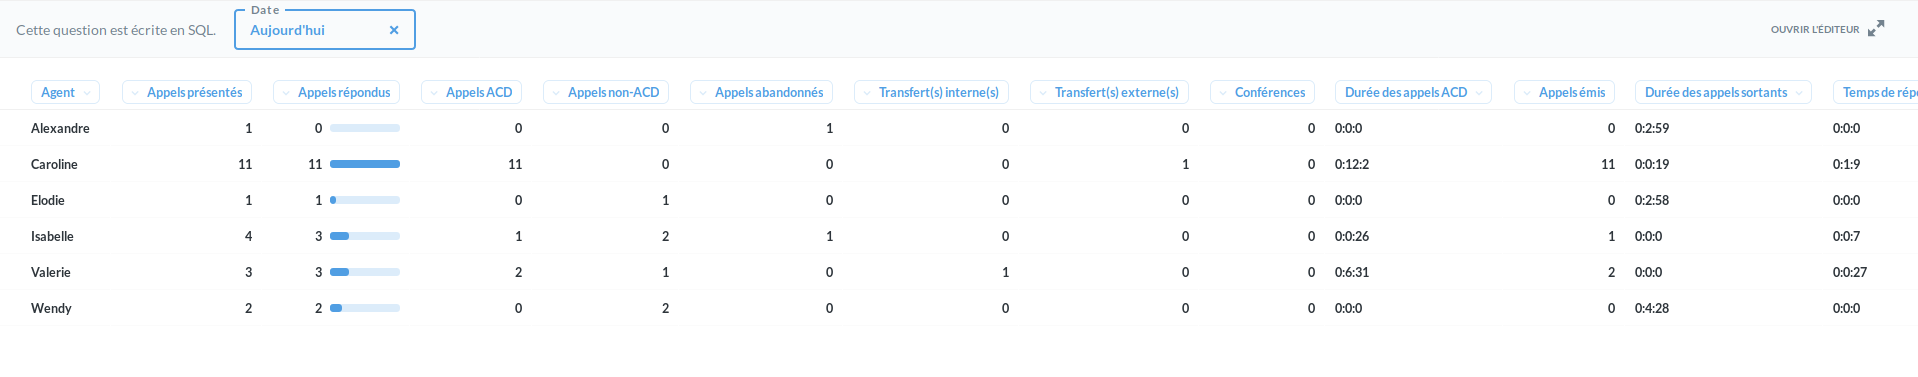
\includegraphics[width=20cm]{image/projet2b.png}
\end{center}
\caption{Photo d'illustration des statiques journaliers}
\label{Photo d'illustration}
\end{figure}

\subsection{Installation du système chez un client}

\paragraph*{}
                   Après avoir réussi à faire sortir ces statiques, mon tuteur présenta cette solution à un client utilisant le même logiciel (Micc). Intéressé qu’il était, le client demanda à avoir cette solution. Il s’agit d’ADEP. Une société d'assurance. 
                   Ayant le même logiciel que celle d’aberia, je n’avais pas à faire d'analyse de base de données. j’ai simplement fait les requêtes qui répondait à leur attentes.
\subsubsection{Statiques demandé par ADEP}
\paragraph{Quotidiennement : histogramme + secteur 3D\newline}
                   Volume d’appels de la journée précédente (global sur toutes files d’attentes) \newline
\begin{itemize}
 \item  Nombre d’agents connectés
                   \item  Nombre d’agents non connectés             
                     \item Appels reçus (par tranche horaire + Histogramme)
                    \item Appels répondus avant attente 20s
                    \item Appels répondus après attente 20s 
                    \item Appels abandonnés (longs)
                    \item Appels débordés GAA (toutes les files d’attentes)
                    \item Appels sortants (volume)
                    \item Performance globale (taux de service)
\end{itemize}

\paragraph*{Hebdomadaire : histogramme + secteur 3D}

\begin{itemize}
 \item Appels de la semaine précédente (par département)
               \item Nombre d’agents connectés par tranche horaire et par département
                 \item Appels reçus (par tranche horaire + histogramme) + choix SVI
                 \item Appels répondus 
                 \item Appels abandonnés
                 \item Appels transférés (autres agents)
                 \item Appels débordés vers GAA (toutes les files d’attentes)
                 \item Performance par département (taux de service) 
                 \item Appels sortants 
\end{itemize}
\paragraph{Mensuel :
    Appels du mois par agent, par file d’attente et par département ( histogramme + secteur 3D)\newline}
    
\begin{itemize}
 \item   Agents connectés durant le mois
     \item   Appels reçus 
      \item    Appels traités
         \item Appels abandonnés
         \item Appels transférés (autres agent ou ligne externe)
        \item Appels débordés GAA
        \item Temps total de connexion par agent
        \item Durée totale de conversation par agent (appels DAA)
        \item Durée totale de conversation par agent sur appels sortants
        \item Choix SVI sur chaque file d’attente
        \item Durée totale d’indisponibilité par agent et par code d’indisponibilité
\end{itemize}

\subsubsection{Résultats}
\paragraph*{}

Les statiques demandé sont belle bien développé et mis en application. 

\begin{figure}[!h]
\begin{center}
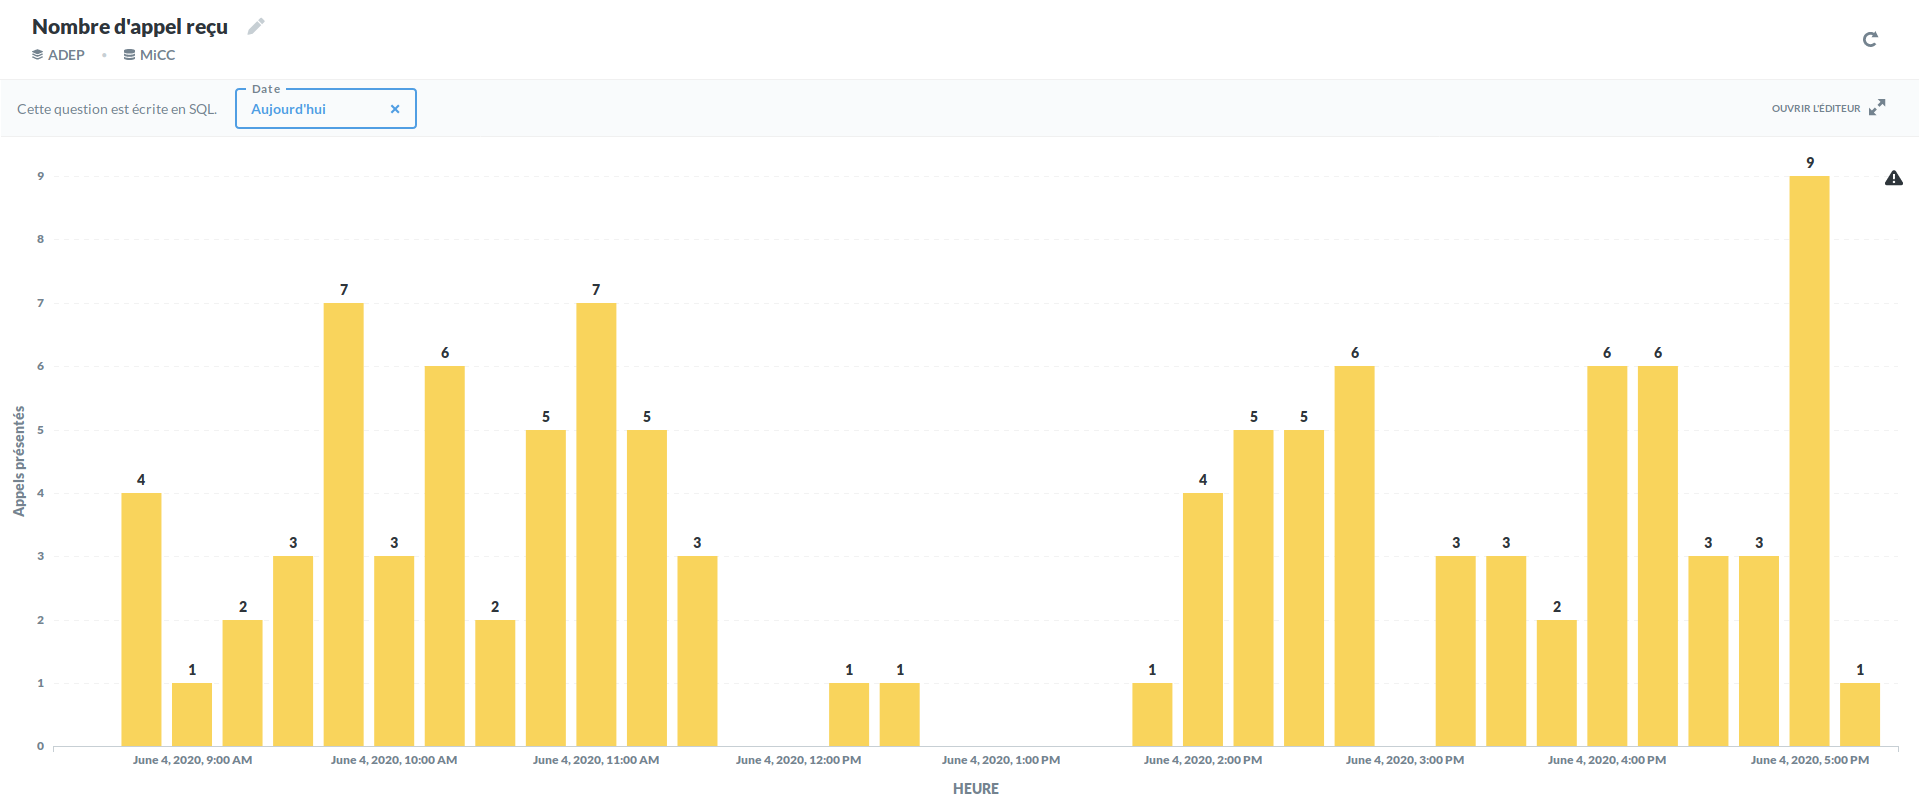
\includegraphics[width=17cm]{image/clienta.png}
\end{center}
\caption{Photo d'illustration des statiques journaliers}
\label{Photo d'illustration}
\end{figure}

\section{Formation des ingénieurs d'Aberia sur Metabase}
\paragraph*{}
Après avoir installer l’outil Metabase, une séance de formation a été organiser entre moi et 5  ingénieurs d’aberia. Je leurs faisais une formation qui a durée 2h sur l’outil. La formation se basait sur l’installation, le paramétrage et la mise en place des requêtes SQL.  En gros, une formation qui leur permettra, dès mon départ de pouvoir continuer les sans problèmes sur la conception des reporting. 

\section{Problèmes rencontrés}
\paragraph{}
              
       D’abord, sur le serveur SQLserver. J’ai, au par avant, utilisé Mysql. Un gestionnaire de base de données. Ils utilisent le même langage de programmation qui est le SQL mais chacun a un certains nombre de commande propre à lui. Ayant l’habitude de travailler sous Mysql, j’ai plongé sur la documentation  de SQLserver afin de voir  les équivalences.\newline 
       
       Ensuite, j’ai eu recours parfois à des notions très poussées de la programmation SQL à savoir les procédures stockées, les vues et la programmations avec des conditions un peu poussé. Ces sont des notions dont j’ignorais l'existence pour certains et embryonnaires  pour  d’autre.
       Pour faire face à cela, j’ai suivi l'intégralité du cours  de SQL  sur Openclassrom (Administrer vos base de données avec Mysql). Ce cours définissait en général les notions de programmation SQL avant d’attaquer directement les  fonctionnalités propre à Mysql. Ainsi à la fin de cours, j’ai développé à la fois des connaissances pointu sur le SQL en général et sur Mysql.
       Après cela, j’ai répondu à toutes les problématiques des notions de procédure stockées et vues qui se sont présentées.

\section{Quelques habitudes adoptées}

\paragraph*{}
       Au cours de mon stage, j’avais pris l’habitude de faire un sauvegarde de mon travail tous les soirs . Même si les requêtes sont conservées  sur le serveur, je faisais attention à mes requêtes qui représentaient le but de mon stage.\newline 
       Je faisais un backup (sauvegarde en jargon informatique) régulier de la base de données qui stockait  les statiques et les requêtes déjà effectuées.\newline 
       Cette technique fortement recommandée et efficace m’a permis de récupérer les travaux de deux semaines après avoir eu une panne sur le serveur. Ce jour là, j’ai eu un problème avec le serveur. Sans le vouloir, j’ai exécuté une commande sur le serveur qui à remis à zéro Metabase. Ayant gardé une sauvegarde, j’ai remonté les informations sur le serveur et tout est revenu à la normal.     
%%%%%%%%%%%%%%%%%%%%%%%%%%%%%%%%%%%%%%%%%%%%%%%%%%%%%%%%%%%%%%%%%%%%%%%%%%       
%                           conclusion 
%%%%%%%%%%%%%%%%%%%%%%%%%%%%%%%%%%%%%%%%%%%%%%%%%%%%%%%%%%%%%%%%%%%%%%%%%%

\section{Conclusion}
\paragraph*{}

        Pour conclure, mon projet consistait à mettre en place un outil de reporting qui faciliterai la supervisions de la qualité de service des services technique, centre d’appel et  commercial. Après avoir adopté des démarches intelligente est cohérentes en accords avec mon tuteur, j’ai finalement réussi à mettre en place l’outil désiré tout en respectant les différents contrainte évoqué. Ce dernier fournis des statiques cohérentes est fiables à l’entreprise, une bonne victoire. Des aujourd’hui, ma solution est mis en avant par Aberia. Elle propose cette plate forme à différents clients et ces derniers sont satisfaits.\newline\newline 
       
       Au cours de stage, j’ai développé des compétences sur plusieurs fronts. À savoir la gestion de projet, la gestion de base de données, le langage SQL  et une esprits d'analyse de données.
       j’ai entre outre développé des compétences importantes sur l'environnement CentOs 7 qui est utiliser par plusieurs entreprise aujourd’hui. j’ai acquis une expérience professionnelles non négligeable et une esprit d’équipe consolidé. j’ai par ailleurs mis en application certaines connaissance qui ne rentrais pas directement dans le cadre de mon projet de stage. Il s’agit du VPN( Virtual Private Network). Étant données que j’ai effectué mon stage en télétravail, j’ai utilisé une connexion VPN pour pouvoir me connecter aux serveur interne de la société. j’ai donc installer le client sur ma machine et mis en œuvre mes connaissances sur ce sujet.\newline\newline     
       
       
       Ce stage m’a ouvert l’esprit sur un domaine que j’aime beaucoup et dont j’y prévois de poursuivre mes études : le Data Analyst. Les différentes analyses de données que j’ai effectué m’ont épanoui de sorte que l’envie de poursuivre mes études ce domaine à fortement augmenter. 
%%%%%%%%%%%%%%%%%%%%%%%%%%%%%%%%%%%%%%%%%%%%%%%%%%%%%%%%%%%%%%%%%%%%%%%%%%%
%                               Annexe
%%%%%%%%%%%%%%%%%%%%%%%%%%%%%%%%%%%%%%%%%%%%%%%%%%%%%%%%%%%%%%%%%%%%%%%%%%%
\appendix
\chapter{Installation de Metabase}

\section*{Installation et configuration de Metabase sur un CentOs7}

\section{Pre-récquis} 

\paragraph*{}
Avant d’installer Metabase, assurez vous  d’avoir installer Java sur votre système. Actuellement, Metabase nécessite Java 8 ou une version supérieur  et fonctionnera soit sur OpenJDK soit sur Oracle JRE.

\paragraph{Installation de JAVA}
\lstset{
language=SQL,
basicstyle=\footnotesize,
}
\begin{lstlisting}
sudo yum install java-1.8.0-openjdk-devel
sudo yum install java-1.8.0-openjdk

\end{lstlisting}

\section{Téléchargement du fichier Jar}

\paragraph*{}
Après cela, nous allons télécharger le fichier jar sur le site officiel de Metabase.\newline\newline 

Créez un dossier Metabase dans /usr/src
Dans ce répertoire, utiliser la commande suivante pour télécharger le fichier : \newline

\lstset{
language=SQL,
basicstyle=\footnotesize,
}
\begin{lstlisting}
wget https://downloads.metabase.com/v0.35.2/metabase.jar
\end{lstlisting}
 (vérifier la version au cas où)  

\paragraph*{}
Dans ce répertoire, vous trouverez  un fichier dont l'extension est .jar . 

Lancement du serveur 

Ainsi, pour lancer le serveur avec ces paramètres par défaut, on utilise la commande suivante :

\lstset{
language=SQL,
basicstyle=\footnotesize,
}
\begin{lstlisting}
java -jar metabase.jar
\end{lstlisting}


\paragraph*{}
Désormais le serveur tourne sur la localhost:3000. C’est, par défaut, le  port utilisé par Metabase.\newline  

\section{Modification des paramètres par défaut}

\paragraph*{} 

Par défaut, Metabase fourni une base de donnée appelé H2. Cette dernière est un fichier.\newline
Arrêtez le serveur, si ce n’est pas encore fait. Rendez-vous sur le dossier Metabase. Vous verrez a part le fichier Metabase.jar d’autres ficher en .db. Ces sont ces fichiers qui continent la base donnée H2 et les différents requêtes que vous avez exécuté.\newline 

Il est possible de faire une migration de ces données vers une base de donnée MYSQL,MARIADB ou POSTGRES. Pour faire cela, la procédure est la suivante.\newline 

\subsection{Migration des données}

\paragraph*{}
Choisissez le type de base de donnée que vous voulez utiliser. En suite exécutez les commandes suivantes(changer les paramètre):
\lstset{
language=SQL,
basicstyle=\footnotesize,
}
\begin{lstlisting}
export MB_DB_TYPE=mysql
export MB_DB_DBNAME=metabase
export MB_DB_PORT=port
export MB_DB_USER=<username>
export MB_DB_PASS=<password>
export MB_DB_HOST=@ip(serveur)
\end{lstlisting}

Après cela , procédez à la migration des données en exécutant la commande suivante : 
\lstset{
language=SQL,
basicstyle=\footnotesize,
}
\begin{lstlisting}
java -jar metabase.jar load-from-h2 /path/to/metabase.db
\end{lstlisting}
\paragraph*{}
Si tout c’est bien passé, vous devrez trouver tout les données dans votre base de données renseignée. Ces paramètre reste valable seulement qu’avec cette session. Une fois que la session sera fermer, les paramètres n’y seront pas. 
 Changement du port et de la taille de JVM
Comme je vous l’avais dit ci-dessus, Metabase marche par défaut sur le port 3000. il est possible de changer ce paramètre en exécutant la commande suivante : \newline
\lstset{
language=SQL,
basicstyle=\footnotesize,
}
\begin{lstlisting}
export MB_JETTY_PORT=num_port
\end{lstlisting}

concernant la taille de la JVM, il suffit de lancer la commande avec les paramètres suivante :
 -Xmx2g. 
Le 2g signifie 2 Go. Vous pouvez mettre la valeurs que vous voulez.    

\subsection{Création d’un service Metabase} 

Jusqu’à présent, le serveur démarre seulement en manuelle. Pour le rendre automatique, vous pouvez créez un service tout en tenant compte des export. Pour ce faire, créez un fichier dans le dossier le dossier metabase(usr/src/metabase/). Insérer tout les variables sans mettre export devant (exemple MB\_\ DB\_\ PASS=<password>). Ensuite, créer le service.

\lstset{
language=SQL,
basicstyle=\footnotesize,
}
\begin{lstlisting}
[Unit]
Description=Metabase demarrage
[Service]
EnvironmentFile= /usr/src/metabase/export_meta
ExecStart=/usr/bin/java -jar -Xmx2g /usr/src/metabase/metabase.jar 
[Install]
WantedBy=multi-user.target

\end{lstlisting} 
À chaque démarrage du server, le fichier export\_ meta sera prise en compte et le serveur travaillera directement sur la base de données.

\chapter{Modelisation de la base de données}

\begin{figure}[!h]
\begin{center}
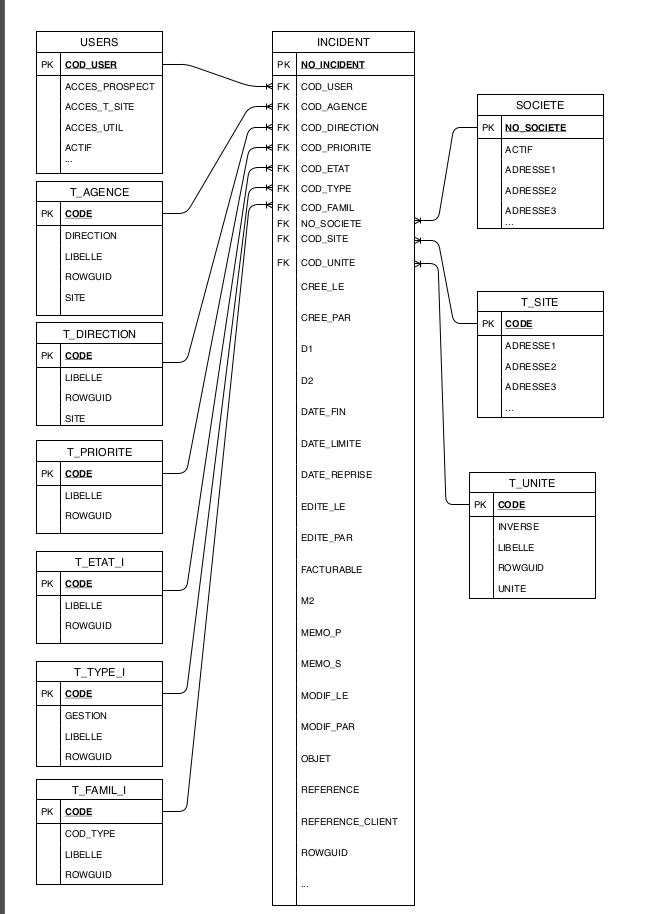
\includegraphics[width=16cm]{image/bdd.png}
\end{center}
\caption{Photo d'illustration des statiques journaliers}
\label{Photo d'illustration}
\end{figure}

\chapter{Requêtes SQL du premier projet}

\subsection{NOMBRE DE TICKETS CRÉÉS}
\lstset{
language=SQL,
basicstyle=\footnotesize,
}
\begin{lstlisting}
SELECT T_PRIORITE.LIBELLE AS PRIORITE, 
COUNT(*) AS NombreIncident 
FROM INCIDENT
INNER JOIN T_PRIORITE
ON 
INCIDENT.COD_PRIORITE=T_PRIORITE.CODE
WHERE {{ANNEE}}
GROUP BY T_PRIORITE.LIBELLE
\end{lstlisting}

\subsection{NOMBRE DE TICKET SUR TECH HOTLINE}
\lstset{
language=SQL,
basicstyle=\footnotesize,
}
\begin{lstlisting}
SELECT COUNT(*) AS NOMBRE_DE_TICKET 
FROM INCIDENT 
WHERE COD_ACTEUR like 'TECH%'
AND COD_ETAT=00
AND {{Date}}
\end{lstlisting}

\subsection{NOMBRE DE TICKETS EN COURS PAR PRIORITÉ} 

\lstset{
language=SQL,
basicstyle=\footnotesize,
}
\begin{lstlisting}
SELECT T_PRIORITE.LIBELLE ,COUNT(*) AS NOMBRE_DE_TIKET_ENCOURS FROM INCIDENT 
INNER JOIN T_PRIORITE
ON 
INCIDENT.COD_PRIORITE=T_PRIORITE.CODE
WHERE COD_ETAT<>03
AND {{DAte}}
GROUP BY T_PRIORITE.LIBELLE
\end{lstlisting}

\subsection{NOMBRE DE TICKET NON SUR TECH HOTLINE} 

\lstset{
language=SQL,
basicstyle=\footnotesize,
}
\begin{lstlisting}
SELECT COUNT(*) AS NOMBRE_DE_TICKET 
FROM INCIDENT 
WHERE COD_ACTEUR like 'TECH%' 
AND {{DATE}}
AND COD_ETAT<>03
\end{lstlisting}



\subsection{NOMBRE DE TICKET EN COURS PAR TECH} 

\lstset{
language=SQL,
basicstyle=\footnotesize,
}
\begin{lstlisting}
SELECT LIB_COM ,COUNT(*) AS NOMBRE_DE_TIKET_ENCOURS 
FROM INCIDENT 
INNER JOIN USERS
ON 
INCIDENT.COD_ACTEUR=USERS.COD_USER
WHERE COD_ETAT<>03
GROUP BY LIB_COM
ORDER BY NOMBRE_DE_TIKET_ENCOURS DESC
\end{lstlisting}


\subsection{NOMBRE DE TICKET RESOLU PAR TECH} 

\lstset{
language=SQL,
basicstyle=\footnotesize,
}
\begin{lstlisting}
SELECT LIB_COM AS TECH,COUNT(*) AS NOMBRE_DE_TICKETS_RESOLU FROM INCIDENT 
INNER JOIN USERS 
ON 
INCIDENT.COD_ACTEUR=USERS.COD_USER
WHERE COD_ETAT=03 
AND {{ANNEE}}
GROUP BY LIB_COM
ORDER BY NOMBRE_DE_TICKETS_RESOLU DESC
\end{lstlisting}

\subsection{TICKETS CLÔTURÉS PAR PAR STATUT} 

\lstset{
language=SQL,
basicstyle=\footnotesize,
}
\begin{lstlisting}
SELECT T_STATUT_ID.LIBELLE AS STATUT,COUNT(*) AS NOMBRE_DE_TICKETS_CLOTURE FROM INCIDENT 
INNER JOIN T_STATUT_ID
ON INCIDENT.COD_STATUT=T_STATUT_ID.CODE
WHERE COD_ETAT=03
AND  {{PERIODE}}
GROUP BY T_STATUT_ID.LIBELLE
ORDER BY STATUT DESC
\end{lstlisting}


\subsection{TOP 10 DES CLIENTS TICKETS CREES} 

\lstset{
language=SQL,
basicstyle=\footnotesize,
}
\begin{lstlisting}
SELECT SOCIETE.NOM, COUNT(*) AS NOMBRE_TICKET FROM INCIDENT
INNER JOIN SOCIETE
ON 
INCIDENT.NO_SOCIETE=SOCIETE.NO_SOCIETE
WHERE  {{PERIODE}} 
GROUP BY SOCIETE.NOM 
order by NOMBRE_TICKET DESC
\end{lstlisting}

\subsection{RELANCES CLIENT} 

\lstset{
language=SQL,
basicstyle=\footnotesize,
}
\begin{lstlisting}
SELECT CONVERT(varchar(20), CREER_LE, 103) AS DATE,COUNT(DISTINCT NO_INCIDENT) AS NOMBRE_DE_RELANCE FROM INFO_INCIDENT 
WHERE {{PERIODE}} 
AND C2='RELANCE PAR LE CLIENT'
GROUP BY CONVERT(varchar(20), CREER_LE, 103)
ORDER BY CONVERT(varchar(20), CREER_LE, 103) 
\end{lstlisting}

\subsection{TOP 10 DES CLIENTS DONT LES TICKETS SONT RÉSOLUS} 

\lstset{
language=SQL,
basicstyle=\footnotesize,
}
\begin{lstlisting}
SELECT TOP 10 SOCIETE.NOM, COUNT(*) AS NOMBRE_TICKET FROM INCIDENT
INNER JOIN SOCIETE
ON 
INCIDENT.NO_SOCIETE=SOCIETE.NO_SOCIETE
WHERE  {{PERIODE}} 
AND COD_ETAT=03
GROUP BY SOCIETE.NOM 
order by NOMBRE_TICKET DESC
\end{lstlisting}

\subsection{NOMBRE DE TICKET DATANT DE DEUX JOURS} 

\lstset{
language=SQL,
basicstyle=\footnotesize,
}
\begin{lstlisting}
SELECT COUNT(*) AS tickets_datant_de_deux_jours from INCIDENT  
WHERE COD_ETAT=00
AND DATEDIFF(day,CREER_LE, SYSDATETIME())=2
\end{lstlisting}
\chapter{Requêtes SQL du deuxième projet}

\subsection{Performance des agents} 

\lstset{
language=SQL,
basicstyle=\footnotesize,
}
\begin{lstlisting}

SELECT AgentFirstName As Agent,
SUM(([AgentNonACDCount])+([AgentACDcount])+[Agentabandoncount]) as 'Appels prEsentes',
SUM(([AgentACDcount])+([AgentNonACDCount])) as Appels rEpondus,
SUM([AgentACDcount]) as 'Appels ACD',
SUM([AgentNonACDCount]) as 'Appels non-ACD',
SUM([Agentabandoncount]) as 'Appels abandonnEs',
SUM([AgentTransferIn]) as 'Transfert(s) interne(s)',
SUM([AgentTransferOut]) as 'Transfert(s) externe(s)',
SUM([AgentConference]) AS 'ConfErences',

CONVERT(VARCHAR(12), SUM(([AgentInternalACDDuration])+([AgentExternalACDDuration]))  / 60 / 60 % 24) 
+ ':' + CONVERT(VARCHAR(2), SUM(([AgentInternalACDDuration])+([AgentExternalACDDuration]))  / 60 % 60) 
+ ':' + CONVERT(VARCHAR(2), SUM(([AgentInternalACDDuration])+([AgentExternalACDDuration])) % 60) AS 'DurEe des appels ACD',

SUM(([AgentExternalACDCount])+([AgentInternalACDCount])) as 'Appels emis',


CONVERT(VARCHAR(12), SUM([AgentOutboundDuration])  / 60 / 60 % 24) 
+ ':' + CONVERT(VARCHAR(2), SUM([AgentOutboundDuration])  / 60 % 60) 
+ ':' + CONVERT(VARCHAR(2), SUM([AgentOutboundDuration])  % 60) AS temps_total_des_appls_sortant,


CONVERT(VARCHAR(12), SUM(([AgentACDTimeToAnswer])+([AgentNonACDTimeToAnswer]))  / 60 / 60 % 24) 
+ ':' + CONVERT(VARCHAR(2), SUM(([AgentACDTimeToAnswer])+([AgentNonACDTimeToAnswer])) / 60 % 60) 
+ ':' + CONVERT(VARCHAR(2), SUM(([AgentACDTimeToAnswer])+([AgentNonACDTimeToAnswer]))  % 60)  AS temps_de_rEponse,

CASE SUM(([AgentNonACDCount])+([AgentACDcount])+([Agentabandoncount]))

WHEN 0 THEN 0 

ELSE (SUM(([AgentACDcount])+([AgentNonACDCount]))*100.0)/SUM(([AgentNonACDCount])+([AgentACDcount])+[Agentabandoncount]) 
END AS Ratio_dEcrochE,

CASE SUM(([AgentNonACDCount])+([AgentACDcount])+[Agentabandoncount])

WHEN 0 THEN 0 

ELSE (SUM([Agentabandoncount])*100.0)/SUM(([AgentNonACDCount])+([AgentACDcount])+[Agentabandoncount])
END AS taux_de_refus

FROM AgentPerformanceByPeriodStats
WHERE {{date}}
GROUP BY ROLLUP(AgentFirstName)

\end{lstlisting}

\subsection{performance des files d'attente}

\lstset{
language=SQL,
basicstyle=\footnotesize,
}
\begin{lstlisting}
SELECT QueueName=IsNull(QueueName,'Total'),

SUM(QueueOffered)as QueueOffered,
SUM(QueueAnswered)as QueueAnswered,
SUM(QueueAbandoned) as QueueAbandoned,
SUM(QueueShortAbandoned) as QueueShortAbandoned,
SUM(QueueInterflowed) as Interflow,
SUM(QueueAnswerByGroup1)as QueueAnswerByGroup1,
SUM(QueueAnswerByGroup2) as QueueAnswerByGroup2,
SUM(QueueAnswerByGroup3) as QueueAnswerByGroup3,
SUM(QueueAnswerByGroup4) as QueueAnswerByGroup4,
SUM(QueueRequeued) as QueueRequeued,
SUM(QueueUnavailable) as Unavailable,

CASE SUM(QueueAnswered)

WHEN 0 THEN 0

ELSE IsNull(SUM(QueueTimeToAnswerTotal) / SUM(QueueAnswered),0)

END AS AvgTTAns

,CASE SUM(QueueAbandoned)

WHEN 0 THEN 0

ELSE IsNull(SUM(QueueTimeToAbandonTotal) / SUM(QueueAbandoned),0)

END AS AvgTTAbd,

CASE SUM(QueueInterflowed)

WHEN 0 THEN 0

ELSE IsNull(SUM(QueueTimeToInterflowTotal) / SUM(QueueInterflowed),0)

END AS AvgTTInt

,CONVERT(VARCHAR(12), SUM(QueueTotalTalkTime)/ 60 / 60 % 24) 
+ ':' + CONVERT(VARCHAR(2), SUM(QueueTotalTalkTime)/ 60 % 60) 
+ ':' + CONVERT(VARCHAR(2), SUM(QueueTotalTalkTime)% 60) 
 AS TotalTalk

,CASE SUM (QueueAnswered)

WHEN 0 THEN 0

ELSE IsNull(SUM(QueueTotalTalkTime) / SUM(QueueAnswered),0)

END AS AvgTalk

,CASE SUM (QueueOffered)

WHEN 0 THEN 0.0

ELSE (CONVERT(float, SUM(QueueAbandoned)) / CONVERT(float, SUM(QueueOffered))) * 100.0

END AS AbdPercentage

,CASE SUM(QueueOffered)

WHEN 0 THEN 100.0

ELSE SUM(convert(float,QueueServiceCount)) / SUM(CONVERT(float, QueueOffered)) * 100.0

END AS ServiceLevel

,CASE SUM(QueueAnswered)

WHEN 0 THEN 0.0

ELSE SUM(CONVERT(float, QueueAnswered)) / SUM(CONVERT(float, QueueOffered)) *100.0

END AS ANSPercentage

FROM QueuePerformanceByPeriodStats

WHERE {{DATE}}
GROUP BY ROLLUP(QueueName)
ORDER by QueueName
\end{lstlisting}



\chapter{Requêtes SQL du troisième projet}
\subsection{Nombre d'appel reçu} 

\lstset{
language=SQL,
basicstyle=\footnotesize,
}
\begin{lstlisting}
SELECT MidnightStartDate AS HEURE,
SUM(([AgentNonACDCount])+([AgentACDcount])+[Agentabandoncount]) as 'Appels prEsentEs'
from AgentPerformanceByPeriodStats
WHERE {{date}}
GROUP by MidnightStartDate        
\end{lstlisting}


\subsection{Appels répondus avant attente 20s} 

\lstset{
language=SQL,
basicstyle=\footnotesize,
}
\begin{lstlisting}
SELECT 
SUM (([AgentACDcount]) + ([AgentNonACDCount])) AS 'Appels rEpondus avant attente 20s'
FROM AgentPerformanceByPeriodStats
WHERE {{DATE}}
AND ([AgentACDTimeToAnswer])< 20 AND ([AgentNonACDTimeToAnswer]) <20        
\end{lstlisting}


\subsection{Agent connecté et non connecté } 

\lstset{
language=SQL,
basicstyle=\footnotesize,
}
\begin{lstlisting}
SELECT COUNT(DISTINCT AgentEventStats.AgentFirstName) as 'agent connectE',
(COUNT(DISTINCT vw_Employee.FirstName)-COUNT(DISTINCT AgentEventStats.AgentFirstName)) as 'agent non connectE'
FROM AgentEventStats,vw_Employee
WHERE {{DATE}}     
\end{lstlisting}
       

\subsection{Appels abandonnés } 

\lstset{
language=SQL,
basicstyle=\footnotesize,
}
\begin{lstlisting}
SELECT SUM(AgentAbandonCount) as 'appls abandones '
FROM AgentPerformanceByPeriodStats
WHERE {{DATE}}  
\end{lstlisting}


\subsection{Débordement GAA} 

\lstset{
language=SQL,
basicstyle=\footnotesize,
}
\begin{lstlisting}
SELECT SUM(QueueInterflowed) as 'dEbordement GAA'
FROM QueuePerformanceByPeriodStats
WHERE {{DATE}}           
\end{lstlisting}


\subsection{Appel émis } 

\lstset{
language=SQL,
basicstyle=\footnotesize,
}
\begin{lstlisting}
SELECT SUM(([AgentExternalACDCount])+([AgentInternalACDCount])) as 'Appels emis' 
FROM AgentPerformanceByPeriodStats
WHERE {{DATE}}
       
\end{lstlisting}


\subsection{Appel répondu } 

\lstset{
language=SQL,
basicstyle=\footnotesize,
}
\begin{lstlisting}
             
SELECT SUM(([AgentACDcount])+([AgentNonACDCount])) as 'Appels rEpondus'
FROM AgentPerformanceByPeriodStats
WHERE {{DATE 
\end{lstlisting}
       
   
\subsection{Appels transféré} 

\lstset{
language=SQL,
basicstyle=\footnotesize,
}
\begin{lstlisting}
SELECT 
SUM(([AgentTransferIn]) +([AgentTransferOut])) as 'Appes TransferEs' 
FROM AgentPerformanceByPeriodStats
WHERE {{DATE}}    
\end{lstlisting}
       

\end{document}

